\chapter{الأمواج الصوتية في الموائع}\label{ch:b2:sound-waves}

عُدَّ الثواني بين الوميض والرعد واقسمها على ثلاثة: فذلك البعد
بالكيلومتر. يقطع الصوت الهواء بثلث كيلومتر في الثانية، والماء
بكيلومتر ونصف، ويوقّت ماسح فوق صوتي الأصداء الآتية من داخل
الجسم إلى جزء من المليون من الثانية ليرسم صورته. وهذا الفصل
يطبّق ميكانيك الموائع في
\cref{ch:b2:euler-bernoulli,ch:b2:fluid-kinematics}
على مائع ساكن تزعجه تموّجة ضغط صغيرة، فيجد \omterm{thm:b2:waves-on-strings:equation}{معادلة دالمبير} من
جديد: \omterm{thm:b2:sound-waves:equation}{سرعة الصوت}، وما الذي يحمل الطاقة، وكم يكون العالي
عاليًا، وكيف ينتشر الصوت في الفضاء، ولماذا تتغير درجة صفارة
وهي تمرّ.

\section{التقريب الصوتي}

\begin{definition}[الاضطراب الصوتي]\label{def:b2:sound-waves:approximation}
\index{تقريب صوتي}\index{فرط الضغط}
مائع ساكن، ضغطه المنتظم $P_0$ وكثافته $\rho_0$، يُزعَج:
$P = P_0 + p(M, t)$، و $\rho = \rho_0 + \rho_1(M, t)$، وسرعته
$\vect v(M, t)$. و\emph{التقريب الصوتي} لا يحتفظ إلا بالمرتبة
الأولى في المقادير الصغيرة $p$ (وهو \emph{فرط الضغط}، أو الضغط
الصوتي) و $\rho_1$ و $\vect v$: أي $|p| \ll P_0$، و $|\rho_1| \ll \rho_0$، و $v \ll c$،
والتحول الذي يخضع له كل \omterm{def:b2:fluid-kinematics:particle}{جسيم مائع} سريع إلى حدّ
لا يتبادل معه أي حرارة: فهو \emph{ثابت الإنتروبيا}، وقابلية
انضغاطه $\chi_S = \frac1\rho\bigl(\frac{\partial\rho}{\partial P}\bigr)_S$.
وتُهمَل الثقالة.
\end{definition}

\begin{theorem}[الأمواج الصوتية]\label{thm:b2:sound-waves:equation}
\index{سرعة الصوت}\index{معادلة الأمواج (صوتيات)}
حتى المرتبة الأولى، تُقرأ \omterm{thm:b2:euler-bernoulli:euler}{معادلة أويلر} وانحفاظ الكتلة وقانون
ثبات الإنتروبيا هكذا
\[
\rho_0\frac{\partial\vect v}{\partial t} = -\operatorname{\vect{grad}}p , \qquad
\frac{\partial\rho_1}{\partial t} + \rho_0\operatorname{div}\vect v = 0 , \qquad
\rho_1 = \rho_0\chi_Sp ,
\]
وهي تعطي معًا \omterm{thm:b2:waves-on-strings:equation}{معادلة الأمواج} من أجل \omterm{def:b2:sound-waves:approximation}{فرط الضغط}،
\[
\Delta p = \frac1{c^2}\frac{\partial^2p}{\partial t^2} , \qquad
c = \frac1{\sqrt{\rho_0\chi_S}} ,
\]
(والمعادلة نفسها من أجل $\rho_1$ و $\vect v$). وفي الغاز المثالي يكون $\chi_S =
1/\gamma P_0$ و
\[
c = \sqrt{\frac{\gamma P_0}{\rho_0}} = \sqrt{\frac{\gamma RT}{M}} :
\]
أي \qty{343}{m/s} في الهواء عند \qty{20}{\degreeCelsius}، وترتفع بمقدار \qty{0.6}{m/s}
في الكلفن؛ و \qty{1000}{m/s} في الهليوم؛ و \qty{1480}{m/s} في الماء ($\chi_S =
\qty{4.5e-10}{Pa^{-1}}$).
\end{theorem}

\begin{proof}
أويلر: الحدّ الحملي $\rho(\vect v\cdot\operatorname{\vect{grad}})\vect v$
من المرتبة الثانية، و $\rho\,\partial_t\vect v \approx \rho_0\,\partial_t\vect v$، و
$\operatorname{\vect{grad}}P = \operatorname{\vect{grad}}p$. والكتلة: $\partial_t\rho +
\operatorname{div}(\rho\vect v) \approx \partial_t\rho_1 + \rho_0\operatorname{div}\vect v$.
وقانون ثبات الإنتروبيا: $\dd\rho = \rho\chi_S\,\dd P$ حتى المرتبة الأولى. ونأخذ
تباعد المعادلة الأولى ومشتق الثانية بالنسبة إلى الزمن:
$\rho_0\partial_t\operatorname{div}\vect v = -\Delta p = -\partial_t^2\rho_1 = -\rho_0\chi_S
\partial_t^2p$. وأما الغاز المثالي، فثبات $PV^\gamma$ على امتداد تحول
ثابت الإنتروبيا يعطي $\dd\rho/\rho = \dd P/\gamma P$، ومنه $\chi_S = 1/\gamma P$،
و $P_0/\rho_0 = RT/M$.
\end{proof}

\begin{remark}[لماذا ثابت الإنتروبيا]\label{rem:b2:sound-waves:laplace}
حسب نيوتن \omterm{thm:b2:sound-waves:equation}{سرعة الصوت} بقابلية الانضغاط عند ثبات الحرارة،
$\sqrt{P_0/\rho_0} = \qty{290}{m/s}$، وهي أدنى بنسبة $15\%$؛ ورأى لابلاس أن
الانضغاطات أسرع من أن تجري الحرارة بين الذرى الدافئة
والقيعان الباردة --- إذ تنتشر الحرارة في دور واحد بضعة ميكرومترات
(\cref{ch:b2:heat-conduction})، وهو لا شيء بالقياس إلى طول الموجة ---
فيكون التحول كظومًا وعكوسًا، ويظهر $\gamma$.
وهكذا تكون \omterm{thm:b2:sound-waves:equation}{سرعة الصوت} قياسًا مباشرًا للمقدار $\gamma$: أي $1.40$ في
الهواء، و $1.67$ في الأرغون.
\end{remark}

\begin{omfigure}
\begin{tikzpicture}[font=\small, x=1cm, y=1cm, >=Stealth]
  \begin{scope}
    \draw[thick] (-3.2,-0.8) rectangle (3.2,0.8);
    \fill[omDef!25] (-0.6,-0.8) rectangle (0.6,0.8);
    \fill[omDef!8] (-0.35,-0.8) rectangle (0.95,0.8);
    \draw[omDef, dashed] (-0.35,-0.8) -- (-0.35,0.8) (0.95,-0.8) -- (0.95,0.8);
    \draw[omThm, very thick, ->] (-1.6,0) -- (-0.65,0) node[above, font=\footnotesize, pos=0.3] {$P(x)S$};
    \draw[omThm, very thick, ->] (1.6,0) -- (0.65,0) node[above, font=\footnotesize, pos=0.3] {$P(x+\dd x)S$};
    \node[font=\footnotesize] at (-0.6,-1.1) {$x$}; \node[font=\footnotesize] at (0.65,-1.1) {$x + \dd x$};
    \draw[omDef, ->] (-0.6,1.05) -- (-0.35,1.05) node[above, font=\footnotesize, pos=1.4] {$\xi(x)$};
    \node[font=\footnotesize] at (0,-1.7) {$\rho_0\,\partial_t v = -\partial_x p$, \quad $\rho_1 = -\rho_0\,\partial_x\xi = \rho_0\chi_S\,p$};
  \end{scope}
  \begin{scope}[xshift=8.2cm]
    \foreach \x in {-2.6,-2.45,...,2.6} {
      \pgfmathsetmacro{\d}{0.18*sin(deg(2.4*\x))}
      \draw[omDef, thick] ({\x+\d},-0.8) -- ({\x+\d},0.8);
    }
    \node[font=\scriptsize] at (-1.6,-1.1) {انضغاط}; \node[font=\scriptsize] at (0,-1.1) {تخلخل}; \node[font=\scriptsize] at (1.6,-1.1) {انضغاط};
    \draw[omThm, thick, ->] (-0.4,1.1) -- (0.8,1.1) node[right, font=\footnotesize] {$c$};
    \node[font=\footnotesize] at (0,-1.7) {موجة صوتية مستوية: تتزاحم شرائح المائع وتتباعد};
  \end{scope}
\end{tikzpicture}

{\small على اليسار: شريحة مائع منتقلة بالمقدار $\xi(x, t)$ ومدفوعة
بالضغطين على وجهيها؛ وانضغاطها يحدّد \omterm{def:b2:sound-waves:approximation}{فرط الضغط}.
وعلى اليمين: موجة صوتية مستوية --- مناطق انضغاط وتخلخل
متناوبة تتحرك بالسرعة $c$، والمائع نفسه يتذبذب جيئةً وذهابًا
على امتداد جهة الانتشار (أي \omterm{prop:b2:waves-on-strings:chain}{موجة طولية}).}
\end{omfigure}

\section{الأمواج المستوية والممانعة والشدّة}

\begin{proposition}[الموجة الصوتية المستوية المتقدمة]\label{prop:b2:sound-waves:plane}
\index{ممانعة صوتية}\index{شدة صوتية}\index{كثافة الطاقة (صوتية)}
من أجل موجة مستوية $p = f(x - ct)$ تنتقل نحو $+x$، تكون سرعة
المائع على امتداد $x$، في طور \omterm{def:b2:sound-waves:approximation}{فرط الضغط}، ويكون
\[
p = Z\,v , \qquad Z = \rho_0c = \sqrt{\rho_0/\chi_S} ,
\]
حيث $Z$ هي \emph{\omterm{prop:b2:sound-waves:plane}{الممانعة الصوتية}} للوسط
(\unit{kg.m^{-2}.s^{-1}}): أي \qty{410}{kg.m^{-2}.s^{-1}} للهواء، و \qty{1.5e6}{kg.m^{-2}.s^{-1}}
للماء، و $\sim\qty{1.6e6}{kg.m^{-2}.s^{-1}}$ للنسيج الرخو،
و \qty{4e7}{kg.m^{-2}.s^{-1}} للفولاذ. وتحمل الموجة كثافة الطاقة
والشدّة (أي الاستطاعة في واحدة المساحة، نحو $+x$)
\[
e = \tfrac12\rho_0v^2 + \tfrac12\chi_Sp^2 , \qquad I = p\,v ,
\]
وهما تحققان $\partial_te + \partial_xI = 0$؛ وفي الموجة المتقدمة يتساوى
نصفا $e$ ويكون $I = p^2/Z = Zv^2$. وموجة جيبية سعة
ضغطها $p_m$ لها الشدّة الوسطى $\langle I\rangle = p_m^2/2Z$.
\end{proposition}

\begin{proof}
من أجل $p = f(x - ct)$، $\rho_0\partial_tv = -\partial_xp = f'/c\cdot c\dots$: وبالضبط،
$\rho_0\partial_tv = -f'(x - ct)$، ويحققها $v = f(x - ct)/\rho_0c$. والحدّ
الكامن في $e$ هو الشغل المخزَّن في ضغط المائع
(إذ انضغاط ثابت الإنتروبيا لواحدة الحجم بالمقدار $\dd V/V = -\chi_S\,\dd p$
يخزّن $\int p\,\chi_S\dd p = \tfrac12\chi_Sp^2$)؛ و $I$ هو معدل شغل قوة
الضغط $pS$ على المائع الذي أمامه، وهو يتحرك بالسرعة $v$، في واحدة المساحة.
والموازنة: $\partial_te = \rho_0v\partial_tv + \chi_Sp\partial_tp = -v\partial_xp - p\partial_xv =
-\partial_x(pv)$ بالمعادلتين المخطَّيتين.
\end{proof}

\begin{definition}[مستوى الصوت]\label{def:b2:sound-waves:decibel}
\index{ديسيبل}\index{مستوى الصوت}\index{عتبة السمع}
\emph{مستوى الصوت} لموجة شدّتها الوسطى $I$ هو
\[
L = 10\log_{10}\frac I{I_0} \ \text{dB} , \qquad I_0 = \qty{1e-12}{W/m^2}
\]
--- وهي عتبة السمع عند \qty{1}{kHz}، وتوافق في الهواء
سعة الضغط $p_0 \approx \qty{2e-5}{Pa}$ (فعّالة) $= 2 \times 10^{-10}$ من
الضغط الجوي. ومضاعفة الشدّة تضيف \qty{3}{dB}؛ وعشرة أضعافها \qty{10}{dB}؛
ومئة ضعف في سعة الضغط \qty{40}{dB}. والغرفة الهادئة
\qty{30}{dB}، والحديث \qty{60}{dB}، والشارع المزدحم \qty{80}{dB}، وحفلة الروك
\qty{110}{dB}، والألم \qty{120}{dB} ($I = \qty{1}{W/m^2}$، و $p_m = \qty{29}{Pa}$).
\end{definition}

\begin{example}[كم يكون الصوت صغيرًا]\label{ex:b2:sound-waves:small}
عند العتبة، وعند \qty{1}{kHz}: $p_m = \qty{2.8e-5}{Pa}$، و $v_m = p_m/Z =
\qty{7e-8}{m/s}$، وسعة الانتقال $\xi_m = v_m/\omega =
\qty{1e-11}{m}$ --- أي عُشر قطر ذرة: فطبلة الأذن تكشف
حركات أصغر من ذرة. وعند \qty{120}{dB} يكون $\xi_m = \qty{11}{\micro m}$،
وهو غير مرئي كذلك، و $p_m/P_0 = 3 \times 10^{-4}$: فحتى أعلى الأصوات
اضطرابات ضئيلة، ولهذا تعمل النظرية الخطية بهذا الإحكام.
\end{example}

\begin{omfigure}
\begin{tikzpicture}
\begin{axis}[omaxis, axis x line=middle, axis y line=left, width=7.4cm, height=4.2cm,
    xlabel={$x$}, ylabel={}, xmin=0, xmax=6.6, ymin=-1.3, ymax=1.4, xtick=\empty, ytick=\empty, samples=100,
    xlabel style={at={(axis description cs:1.0,0.5)}, anchor=west},
    legend style={font=\scriptsize, at={(0.5,1.02)}, anchor=south, legend columns=3, draw=none, fill=none}]
  \addplot[omThm, thick, domain=0:6.28] {sin(deg(x))};
  \addplot[omDef, thick, dashed, domain=0:6.28] {sin(deg(x))};
  \addplot[omProp, thick, domain=0:6.28] {cos(deg(x))};
  \legend{$p$, $v = p/Z$, $\xi$}
\end{axis}
\end{tikzpicture}
\hfill
\begin{tikzpicture}[font=\small, x=1cm, y=1cm, >=Stealth]
  \draw[thick, ->] (0,0) -- (0,4.4);
  \foreach \l/\t in {0/عتبة السمع, 1/حفيف الأوراق, 2/غرفة هادئة, 3/حديث, 4/شارع مزدحم, 5/شاحنة على \qty{10}{m}, 6/حفلة روك, 7/الألم} {
    \pgfmathsetmacro{\y}{0.6*\l}
    \draw (-0.1,\y) -- (0.1,\y);
    \node[anchor=east, font=\scriptsize] at (-0.15,\y) {\pgfmathparse{int(20*\l)}\pgfmathresult~dB};
    \node[anchor=west, font=\scriptsize] at (0.15,\y) {\t};
  }
  \node[font=\scriptsize, anchor=south] at (0,4.45) {$I$ ($\times 100$ في كل درجة)};
\end{tikzpicture}

{\small على اليمين: في الموجة الصوتية المستوية المتقدمة يكون \omterm{def:b2:sound-waves:approximation}{فرط
الضغط} وسرعة المائع في طور واحد، ويتأخر الانتقال بربع
دور. وعلى اليسار: سلّم \omterm{def:b2:sound-waves:decibel}{الديسيبل} --- فكل درجة \qty{20}{dB} تضرب
الشدّة بمئة وسعة الضغط بعشرة.}
\end{omfigure}

\section{الأمواج الكروية}

\begin{proposition}[الأمواج الكروية وقانون التربيع العكسي]\label{prop:b2:sound-waves:spherical}
\index{موجة كروية}\index{قانون التربيع العكسي (الصوت)}
منبع صغير يشعّ بالتساوي في كل الاتجاهات ينتج \omterm{prop:b2:sound-waves:spherical}{الموجة
الكروية}
\[
p(r, t) = \frac{A}{r}\,f\Bigl(t - \frac rc\Bigr) ,
\]
وتهبط سعتها مثل $1/r$ وتهبط شدّتها مثل $1/r^2$:
فمن أجل منبع استطاعته الصوتية $\mathcal P$ يكون $I = \mathcal P/4\pi r^2$، أي
$-\qty{6}{dB}$ كلما تضاعف البعد. وبعيدًا عن المنبع تكون
الموجة مستوية موضعيًّا، و $v = p/Z$ قطرية.
\end{proposition}

\begin{proof}
بالإحداثيات الكروية، من أجل دالة في $r$ وحدها، $\Delta p =
\frac1r\frac{\partial^2(rp)}{\partial r^2}$ (مسلَّم بها؛ \cref{ch:b2:maxwell-equations})،
ومنه يحقق $u = rp$ \omterm{thm:b2:waves-on-strings:equation}{معادلة الأمواج} ذات البعد الواحد $\partial_r^2u = \partial_t^2u/c^2$،
ومنه $u = Af(t - r/c)$ من أجل الموجة الخارجة. والاستطاعة العابرة
لكرة نصف قطرها $r$ هي $4\pi r^2I$، وهي ثابتة إن لم يُمتصّ شيء.
\end{proof}

\begin{example}[صفارة وحديث]\label{ex:b2:sound-waves:siren}
صفارة استطاعتها \qty{10}{W}: $I = 10/4\pi r^2$، أي \qty{0.8}{W/m^2} عند \qty{1}{m} (و \qty{119}{dB}،
أي ألم)، و \qty{79}{dB} عند \qty{100}{m}، و \qty{59}{dB} عند \qty{1}{km} --- ولا تزال مسموعة فوق
المدينة. ويشعّ الصوت البشري نحو \qty{10}{\micro W}: أي \qty{60}{dB} عند \qty{1}{m}،
و \qty{40}{dB} عند \qty{10}{m}. ويمتصّ الهواء الصوت أيضًا (وأكثر عند
التواترات العالية، بضعة ديسيبلات في المئة متر عند \qty{10}{kHz})، ولهذا
يهدر الرعد البعيد هديرًا خفيضًا.
\end{example}

\section{أثر دوبلر}

\begin{theorem}[أثر دوبلر]\label{thm:b2:sound-waves:doppler}
\index{أثر دوبلر}
منبع يبثّ عند التواتر $f$ ويتحرك بالسرعة $v_s$ على امتداد
المستقيم الواصل بينه وبين راصد يتحرك بالسرعة $v_o$، والسرعتان
موجبتان حين يتقاربان؛ وينتقل الصوت بالسرعة $c$ في
الهواء الساكن. ويتلقى الراصد التواتر
\[
f' = f\,\frac{c + v_o}{c - v_s} .
\]
فالمنبع المتحرك يزاحم جبهات موجته أمامه ($\lambda' = (c - v_s)/f$)
ويباعدها خلفه؛ والراصد المتحرك يلقى جبهات الموجة
بالمعدل $(c + v_o)/\lambda$. ومن أجل $v_s, v_o \ll c$ يعطي الاثنان $\Delta f/f \approx
(v_s + v_o)/c$.
\end{theorem}

\begin{proof}
المنبع المتحرك: تفترق جبهتا الموجة المبثوثتان عند $t$ و $t + 1/f$
بالمقدار $c/f - v_s/f$ في جهة الحركة، ومنه يكون طول الموجة أمامه
$\lambda' = (c - v_s)/f$ ويكون التواتر الذي يتلقاه راصد ثابت
$c/\lambda'$. والراصد المتحرك: طول الموجة $\lambda = c/f$ لكن الجبهات تمرّ
بالسرعة النسبية $c + v_o$. ثم نجمع بينهما.
\end{proof}

\begin{omfigure}
\begin{tikzpicture}[font=\small, x=1cm, y=1cm, >=Stealth]
  \begin{scope}
    \foreach \i in {0,1,2,3,4} {
      \pgfmathsetmacro{\r}{0.45*(5-\i)}
      \pgfmathsetmacro{\cx}{0.27*\i-0.23}
      \draw[omDef, thick] (\cx,0) circle (\r);
    }
    \fill[omThm] (1.12,0) circle (2pt);
    \draw[omThm, thick, ->] (1.12,0.15) -- (1.9,0.15) node[above, font=\footnotesize] {$v_s$};
    \node[font=\footnotesize] at (2.0,-2.45) {أمامه: $\lambda' < \lambda$};
    \node[font=\footnotesize] at (-1.5,-2.45) {خلفه: $\lambda' > \lambda$};
    \node[font=\footnotesize] at (0.4,-3.2) {$f' = f\,\dfrac{c + v_o}{c - v_s}$};
  \end{scope}
  \begin{scope}[xshift=8.2cm]
    \foreach \i in {0,1,2,3,4} {
      \pgfmathsetmacro{\r}{0.4*(5-\i)}
      \pgfmathsetmacro{\cx}{0.6*\i-1.12}
      \draw[omDef, thick] (\cx,0) circle (\r);
    }
    \fill[omThm] (1.88,0) circle (2pt);
    \draw[omThm, thick, ->] (1.88,0.15) -- (2.7,0.15) node[above, font=\footnotesize] {$v > c$};
    \draw[omProp, thick] (1.88,0) -- (-0.36,2.0); \draw[omProp, thick] (1.88,0) -- (-0.36,-2.0);
    \draw (0.9,0) arc[start angle=180, end angle=138, radius=0.98] node[left, font=\footnotesize, xshift=-1pt] {$\theta$};
    \node[font=\footnotesize] at (0.3,-3.2) {مخروط ماخ: $\sin\theta = c/v$};
  \end{scope}
\end{tikzpicture}

{\small على اليسار: تتزاحم جبهات موجة منبع متحرك أمامه وتتباعد
خلفه --- فالدرجة أحدّ وهو مقبل، وأخفض وهو مدبر. وعلى اليمين: منبع
أسرع من الصوت يترك جبهات موجته خلفه؛ وغلافها هو
\omterm{rem:b2:sound-waves:mach}{مخروط ماخ}، ويُسمع على الأرض دويًّا.}
\end{omfigure}

\begin{example}[الصفارات ومسدسات الرادار والكريات الحمراء]\label{ex:b2:sound-waves:dopplerex}
صفارة إسعاف عند \qty{700}{Hz} تمرّ بسرعة \qty{25}{m/s}: تُسمع \qty{755}{Hz}
وهي مقبلة، و \qty{651}{Hz} وهي مدبرة --- أي هبوط بسدس ديوان،
وهو انخفاض الصفارة المألوف. ويقيس مسدس رادار الشرطة الأثر
نفسه على موجة راديوية عند \qty{24}{GHz} تنعكس عن سيارة (فالموجة
تنزاح مرتين، بتلقي السيارة لها وإعادة بثّها): $\Delta f = 2fv/c =
\qty{4.8}{kHz}$ عند \qty{30}{m/s}. ومسبار فوق صوتي عند \qty{5}{MHz} مصوَّب إلى
شريان يسمع كريات الدم عند $\Delta f = 2fv\cos\theta/c \approx \qty{1.6}{kHz}$
من أجل \qty{0.5}{m/s} عند \qty{60}{\degree}: أي صفير مسموع درجته سرعة
الدم. وتنزاح الخطوط الطيفية لمجرّة مدبرة نحو
الأحمر بالمقدار $\Delta\lambda/\lambda = v/c$ --- والصيغة صحيحة في الضوء عند السرعات الصغيرة،
مع التصحيح النسبوي فيما وراءها.
\end{example}

\begin{remark}[فوق سرعة الصوت]\label{rem:b2:sound-waves:mach}
\index{مخروط ماخ}\index{دويّ صوتي}
حين $v_s > c$ تنهار الصيغة ($f' < 0$ أمامه): فلا صوت يسبق
المنبع. ولجبهات الموجة المبثوثة على امتداد المسار غلاف
مخروطي نصف زاويته $\theta$ حيث $\sin\theta = c/v_s$ (وهو \emph{\omterm{rem:b2:sound-waves:mach}{مخروط ماخ}})؛
وقفزة الضغط التي يحملها المخروط هي \omterm{rem:b2:sound-waves:mach}{الدويّ الصوتي}، ولا يبلغ
سامعًا على الأرض إلا بعد مرور الطائرة --- فعند
ماخ $2$ وارتفاع \qty{10}{km} يكون $\theta = \qty{30}{\degree}$ ويصل الدويّ
بعد المرور فوق الرأس بمقدار $10\,\text{km}/\tan\theta/v_s \approx \qty{25}{s}$.
وطرقة الرصاصة وطرف السوط هما المخروط نفسه.
\end{remark}

\begin{method}[رتب القدر في الصوتيات]\label{met:b2:sound-waves:method}
إذا أُعطي \omterm{def:b2:sound-waves:decibel}{مستوى الصوت} $L$: فإن $I = I_0\,10^{L/10}$؛ ثم $p_m = \sqrt{2ZI}$،
و $v_m = p_m/Z$، و $\xi_m = v_m/\omega$؛ واستطاعة المنبع $4\pi r^2I$ إن كان
يشعّ في كل الاتجاهات (وأقل بمرتين فوق أرض صلبة، فهي
تعكس في نصف فضاء). والانتقال من $r_1$ إلى $r_2$ يغير $L$ بالمقدار
$20\log_{10}(r_1/r_2)$. وجمع $n$ منبعًا متساويًا غير مترابط يضيف
$10\log_{10}n$؛ ومنبعان مترابطان في طور واحد عند نقطة يضيفان \qty{6}{dB}.
\end{method}

\section{تمارين}

\begin{exercise}[$\star$]\label{exo:b2:sound-waves:1}
\omterm{thm:b2:sound-waves:equation}{سرعة الصوت} في الهواء ($\gamma = 1.40$، و $M = \qty{29}{g/mol}$) عند
\qty{0}{\degreeCelsius} و \qty{20}{\degreeCelsius} وعند \qty{-50}{\degreeCelsius}
(أي على ارتفاع \qty{10}{km})؛ وفي الهليوم ($\gamma = 1.67$، و $M = \qty{4}{g/mol}$) وفي
ثاني أكسيد الكربون ($\gamma = 1.30$، و $M = \qty{44}{g/mol}$) عند \qty{20}{\degreeCelsius}.
ولماذا يبدو الصوت حادًّا بعد استنشاق الهليوم؟
\end{exercise}

\begin{exercise}[$\star$]\label{exo:b2:sound-waves:2}
حديث عند \qty{60}{dB} و \qty{500}{Hz}: أوجد الشدّة، وسعة الضغط،
وسعة السرعة، وسعة الانتقال في الهواء
($Z = \qty{410}{kg.m^{-2}.s^{-1}}$). والأمر نفسه من أجل \qty{120}{dB}. ومستوى شخصين
يتكلمان معًا؛ ومئة شخص.
\end{exercise}

\begin{exercise}[$\star$]\label{exo:b2:sound-waves:3}
مكبر صوت يشعّ \qty{1.0}{W} من الصوت بالتساوي في كل الاتجاهات.
أوجد الشدّة والمستوى عند \qty{1}{m} و \qty{10}{m} و \qty{100}{m}؛ والبعد الذي
يهبط عنده المستوى إلى \qty{60}{dB}؛ والاستطاعة اللازمة من أجل \qty{100}{dB} عند \qty{30}{m}
(أي حفلة في الهواء الطلق).
\end{exercise}

\begin{exercise}[$\star$]\label{exo:b2:sound-waves:4}
يُسمع الرعد بعد الوميض بمقدار \qty{4.5}{s}: أوجد البعد. وترتدّ صفارة سفينة
عن جرف بعد \qty{3.0}{s}: أوجد البعد. والسونار: يعود صدى من
قاع البحر بعد \qty{2.4}{s} ($c = \qty{1500}{m/s}$): أوجد العمق. ويعود صدى
فوق صوتي عند \qty{5}{MHz} بعد \qty{130}{\micro s} في نسيج
(\qty{1540}{m/s}): أوجد العمق.
\end{exercise}

\begin{exercise}[$\star\star$]\label{exo:b2:sound-waves:5}
صفارة قطار عند \qty{500}{Hz}؛ و $c = \qty{340}{m/s}$. (أ) أوجد التواتر الذي يسمعه
شخص على الرصيف والقطار مقبل بسرعة \qty{40}{m/s}، ثم
بعد مروره. (ب) والشخص في قطار يتحرك نحو
الصفارة بسرعة \qty{40}{m/s} والصفارة ساكنة؛ ثم يتحرك الاثنان أحدهما
نحو الآخر بسرعة \qty{40}{m/s}: قارن بسرعة نسبية \qty{80}{m/s} و
جسم واحد ساكن. (ج) والتواتر الذي يسمعه سائق قطار الصفارة
من الصدى عن جدار أمامه.
\end{exercise}

\begin{exercise}[$\star\star$]\label{exo:b2:sound-waves:6}
من أجل سعة ضغط \qty{1.0}{Pa} عند \qty{1}{kHz}، احسب
سعتي السرعة والانتقال، والشدّة والمستوى في
الهواء، وفي الماء ($Z = \qty{1.5e6}{kg.m^{-2}.s^{-1}}$)، وفي الفولاذ
($\qty{4e7}{kg.m^{-2}.s^{-1}}$). فالضغط نفسه والشدّات مختلفة جدًّا:
علّق. (وتُذكر المستويات تحت الماء بالنسبة إلى \qty{1}{\micro Pa}: فكم تكون
\qty{1}{Pa} على ذلك السلّم؟)
\end{exercise}

\begin{exercise}[$\star\star$]\label{exo:b2:sound-waves:7}
(أ) سرعة نيوتن عند ثبات الحرارة $\sqrt{P_0/\rho_0}$ من أجل الهواء عند
\qty{20}{\degreeCelsius} ($\rho_0 = \qty{1.20}{kg/m^3}$) وتصحيح لابلاس.
(ب) والمقيس: \qty{343}{m/s} في الهواء، و \qty{323}{m/s} في الأرغون ($M = \qty{40}{g/mol}$)
عند \qty{20}{\degreeCelsius}: استنتج $\gamma$ لكل منهما؛ وفسّر ذلك بعدد
درجات الحرية. (ج) وقدّر إلى أي بعد تنتشر الحرارة في
دور واحد عند \qty{1}{kHz} (وانتشارية الهواء الحرارية
\qty{2e-5}{m^2/s}) وقارنه بطول الموجة.
\end{exercise}

\begin{exercise}[$\star\star$]\label{exo:b2:sound-waves:8}
\emph{أنابيب الأرغن.} في أنبوب ينعدم \omterm{def:b2:sound-waves:approximation}{فرط الضغط} عند طرف مفتوح
وتنعدم السرعة عند طرف مغلق. (أ) الأمواج المستقرة في أنبوب
مفتوح من طرفيه: بيّن أن أنماطه $f_n = nc/2L$؛ وفي أنبوب مغلق من
طرف واحد، $f_n = (2n - 1)c/4L$. (ب) الأطوال اللازمة لنمط أساسي عند \qty{440}{Hz}
في كل حالة. (ج) وأي التوافقيات يحويها كل أنبوب؟ (د) والطرف
المفتوح الحقيقي يقع على نحو $0.6$ من نصف القطر خلف الأنبوب (تصحيح الطرف): ومن أجل
أنبوب طوله \qty{4}{cm}، أوجد التصحيح على $L$ وعلى $f$.
\end{exercise}

\begin{exercise}[$\star\star$]\label{exo:b2:sound-waves:9}
صفارة كهربائية استطاعتها \qty{2.0}{kW} تحوّل $20\%$ من استطاعتها إلى صوت
مشعّ في نصف فضاء (فهي على سطح). (أ) أوجد الشدّة والمستوى
وسعة الضغط عند \qty{100}{m}. (ب) وبعد عتبة الألم
(\qty{120}{dB})؛ وبعد الخط الكفافي عند \qty{70}{dB} حيث تكفّ عن الإنذار.
(ج) ويضيف امتصاص الهواء \qty{1}{dB} في كل \qty{100}{m} عند تواترها:
أوجد بعد الخط الكفافي عند \qty{70}{dB} الآن (حُلّ عدديًّا). (د) وكم
صفارة كهذه تغطي مدينة نصف قطرها \qty{10}{km}؟
\end{exercise}

\begin{exercise}[$\star\star\star$]\label{exo:b2:sound-waves:10}
\emph{طاقة موجة صوتية مستقرة.} في أنبوب مغلق طوله $L$
يكون \omterm{def:b2:sound-waves:approximation}{فرط الضغط} $p = p_m\cos(kx)\cos(\omega t)$، و $k = n\pi/L$. (أ) أوجد $v(x,
t)$ من \omterm{thm:b2:euler-bernoulli:euler}{معادلة أويلر} المخطَّاة. (ب) كثافتي الطاقة الحركية
والكامنة؛ وبيّن أنهما تتذبذبان في تربيع الطور زمنيًّا
وتنزاحان بربع طول موجة مكانيًّا. (ج) الطاقة الكلية في
الأنبوب (ومقطعه $S$)؛ وتحقق من أنها ثابتة. (د) الشدّة الوسطى:
معدومة في كل مكان --- ومع ذلك تتحرك الطاقة: فصف كيف.
\end{exercise}

\begin{exercise}[$\star\star\star$]\label{exo:b2:sound-waves:11}
\emph{\omterm{rem:b2:sound-waves:mach}{الدويّ الصوتي}.} تطير طائرة أفقيًّا بالسرعة $v = 1.6\,c$ على
ارتفاع $h = \qty{12}{km}$، و $c = \qty{300}{m/s}$ هناك. (أ) استنتج زاوية
ماخ من غلاف جبهات \omterm{prop:b2:sound-waves:spherical}{الموجة الكروية}. (ب) والزمن بين
المرور فوق الرأس والدويّ على الأرض (بإهمال تغيّر
$c$ مع الارتفاع). (ج) وعرض الشريط على الأرض الذي يسمع
الدويّ وهي تمرّ، إذا سُمع أثر المخروط ضمن
$\pm\qty{30}{km}$ من المسار: ولماذا يُمنع الطيران الأسرع من الصوت
فوق اليابسة؟ (د) ورصاصة بندقية عند \qty{800}{m/s}: أوجد زاوية ماخ؛
وما الذي يسمعه راصد يقف على \qty{10}{m} من المسار، وبأي ترتيب.
\end{exercise}

\begin{exercise}[$\star\star\star$]\label{exo:b2:sound-waves:12}
\emph{الدوبلر فوق الصوتي.} يبثّ مسبار عند $f = \qty{5.0}{MHz}$ في نسيج
($c = \qty{1540}{m/s}$)؛ وتتحرك الكريات الحمراء بالسرعة $v$ على امتداد وعاء يصنع
الزاوية $\theta$ مع الحزمة. (أ) أوجد التواتر الذي تتلقاه كرية (وهي راصد
متحرك). (ب) ثم تعيد بثّ (أي تنثر) هذا التواتر منبعًا متحركًا:
أوجد التواتر العائد إلى المسبار؛ وبيّن أن $\Delta f = 2fv\cos\theta/c$ من أجل $v \ll c$. (ج)
وأوجد $\Delta f$ من أجل $v = \qty{0.50}{m/s}$ و $\theta = \qty{60}{\degree}$؛ ومن أجل $\theta = \qty{90}{\degree}$
--- فماذا يفعل المشغّل؟ (د) والمسبار يميّز \qty{50}{Hz}:
أوجد تمييز السرعة. ولماذا تُجعل إشارة الدوبلر مسموعة لا
معروضة فقط؟
\end{exercise}

\begin{omfigure}
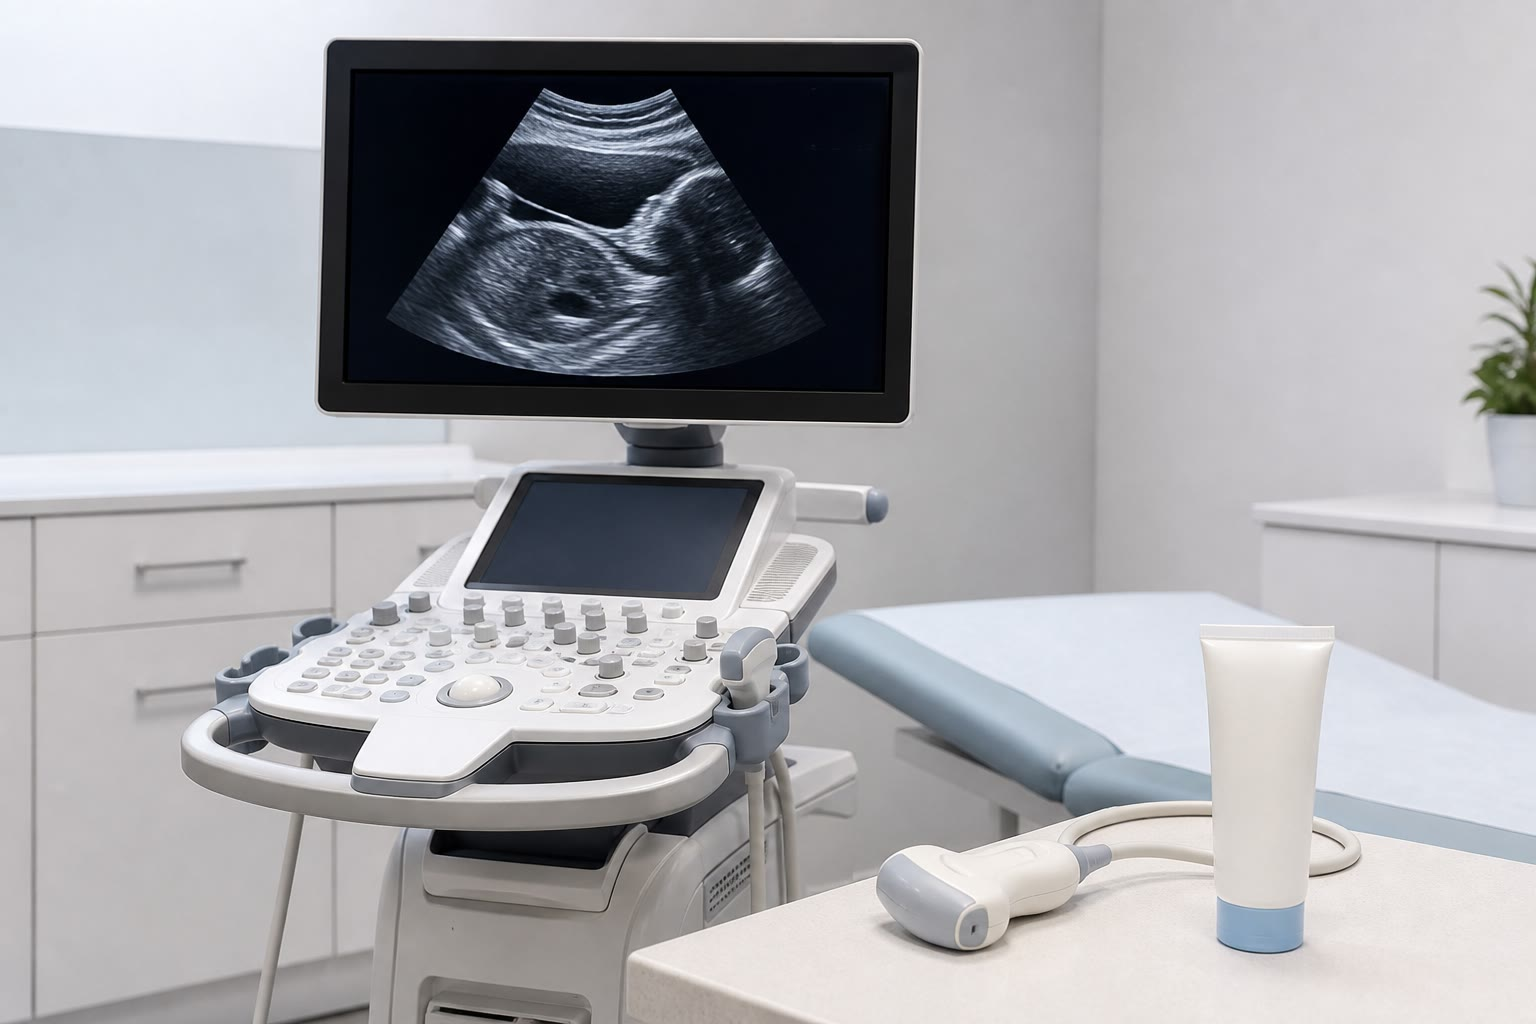
\includegraphics[width=0.58\linewidth]{images/book4/ai/b4-07-ultrasound-probe.jpg}

{\small ماسح فوق صوتي: بضعة ميغاهرتز من الصوت، وأصداء موقَّتة، وعدم توافق الممانعات بين الأنسجة، ترسم الصورة؛ والهلام يزيل غشاء الهواء الذي كان ليعكس كل شيء.}
\end{omfigure}

\section{مسألة: من الرعد إلى جهاز التصوير بالصدى}

\begin{problem}[{مسألة نهاية الأسبوع --- الصوت في الهواء الطلق، وفي قاعة
حفلات، وداخل الجسم، ومن صفارة عابرة}]
\label{pb:b2:sound-waves:1}

الهواء: $\gamma = 1.40$، و $M = \qty{29}{g/mol}$، و $Z = \qty{410}{kg.m^{-2}.s^{-1}}$ عند
\qty{15}{\degreeCelsius}؛ و $R = \qty{8.31}{J/(mol.K)}$.

\medskip
\noindent\textbf{الجزء I --- العاصفة.}
\begin{enumerate}
  \item \omterm{thm:b2:sound-waves:equation}{سرعة الصوت} عند \qty{15}{\degreeCelsius} وعند \qty{30}{\degreeCelsius}؛
        وبرّر قاعدة «ثلاث ثوانٍ في الكيلومتر».
  \item ويصل الرعد بعد الوميض بمقدار \qty{4.0}{s}: أوجد بعد
        الصاعقة. ويدوم الرعد ثوانيَ عدة مع أن الوميض
        لحظي: فلماذا؟
  \item وقرب الصاعقة يبلغ المستوى \qty{120}{dB}: أوجد سعة الضغط
        وسعة سرعة الهواء.
  \item الطاقة المتلقاة في المتر المربع من جدار أثناء قصفة رعد
        مدتها \qty{2}{s} عند \qty{120}{dB}.
  \item وفي ليلة صافية تبرد الأرض ويكون الهواء أبرد في الأسفل
        منه في الأعلى. وتحقق أشعة الصوت قانون سنيل بين الطبقات،
        $\sin i/c = \text{ثابت}$: فهل تنحني الأشعة المرسلة نحو الأعلى نزولًا أم صعودًا؟
        ولماذا تُسمع الأصوات البعيدة بهذا الوضوح ليلًا وفوق الماء؟
  \item وبالنهار العكس: فلا يسمع سامع على بعد \qty{3}{km} شيئًا.
        قدّر الزاوية التي انحنى بها شعاع أفقي بعد
        \qty{3}{km} إذا هبطت $c$ بمقدار \qty{1}{\%} في كل \qty{500}{m} من الارتفاع
        (وعامِل الانحناء منتظمًا: فالشعاع دائرة).

  \item ويمتصّ الهواء التواترات العالية أكثر بكثير من المنخفضة: فلماذا
        يهدر الرعد البعيد بينما تطقطق الصاعقة القريبة؟
\end{enumerate}

\medskip
\noindent\textbf{الجزء II --- الحفلة.}
مكبر صوت يتلقى \qty{100}{W} من الاستطاعة الكهربائية ويحوّل
$2\%$ منها إلى صوت، مشعّ بالتساوي في نصف الفضاء أمامه.
\begin{enumerate}[resume]
  \item الاستطاعة الصوتية؛ والشدّة والمستوى عند \qty{10}{m}.
  \item سعة الضغط هناك؛ وسعتا السرعة والانتقال
        عند \qty{100}{Hz}.
  \item المستوى عند \qty{1}{m} (أهو آمن؟) والبعد الذي تهبط عنده
        الموسيقى إلى \qty{60}{dB}.
  \item وعشرة مكبرات متماثلة موزَّعة حول المسرح، غير
        متوافقة في الطور: أوجد المستوى عند \qty{10}{m}. ومكبران يُغذَّيان في طور
        واحد، وعلى البعد نفسه من سامع على محورهما: أوجد المستوى هناك.
  \item والقاعة (حجمها \qty{10000}{m^3}) فيها \qty{2000}{m^2} من الجدران والجمهور تمتصّ $30\%$ من
        الصوت الذي يصيبها: قدّر الطاقة الصوتية المخزَّنة في
        القاعة عند التوازن وزمن التجاوب (أي الزمن اللازم كي
        يهبط المستوى \qty{60}{dB} بعد توقف الموسيقى)، باستعمال
        الموازنة بين الاستطاعة المبثوثة والاستطاعة الممتصّة
        ($I_{\text{جدار}} \approx ce/4$ في مجال منتشر، مسلَّم بها).
\end{enumerate}

\medskip
\noindent\textbf{الجزء III --- جهاز التصوير بالصدى.}
النسيج الرخو: $c = \qty{1540}{m/s}$، و $Z = \qty{1.6e6}{kg.m^{-2}.s^{-1}}$؛ والعظم
$Z = \qty{7e6}{kg.m^{-2}.s^{-1}}$؛ والهواء $\qty{400}{kg.m^{-2}.s^{-1}}$. وعند الورود
الناظمي تكون سعة الضغط المنعكسة عند سطح فاصل $r = (Z_2 -
Z_1)/(Z_2 + Z_1)$ مضروبةً في الواردة (وهي مشتقّة في
\cref{ch:b2:wave-interfaces})؛ ويوهن النسيج الصوت بنحو
\qty{0.5}{dB} في السنتيمتر وفي الميغاهرتز.
\begin{enumerate}[resume]
  \item طول الموجة في النسيج عند \qty{3}{MHz} و \qty{5}{MHz} و \qty{10}{MHz}؛
        وأصغر تفصيل يستطيع كل منها تمييزه هو نحو طول موجة واحد.
  \item تأخّر الصدى من عضو على عمق \qty{12}{cm}؛ وأعظم معدل يمكن
        إرسال النبضات به دون خلط الأصداء؛ وزمن بناء
        صورة من $200$ سطر.
  \item النسبة المنعكسة من الضغط، ومن الطاقة، عند سطح فاصل بين
        النسيج والهواء؛ وعند سطح فاصل بين النسيج والعظم؛ وبين الشحم
        ($Z = \qty{1.38e6}{kg.m^{-2}.s^{-1}}$) والعضل
        ($\qty{1.70e6}{kg.m^{-2}.s^{-1}}$). ولماذا الهلام، ولماذا ترمي العظام
        ظلالًا؟
  \item وعند \qty{5}{MHz} تعبر الحزمة \qty{2}{cm} من الشحم قبل أن تلقى
        العضل: أوجد النسبة من الطاقة المبثوثة التي تعود إلى
        المسبار من ذلك السطح الفاصل (الانعكاس ووهن الذهاب
        والإياب)، \omterm{def:b2:sound-waves:decibel}{بالديسيبل}.
  \item وهن الذهاب والإياب \omterm{def:b2:sound-waves:decibel}{بالديسيبل} من أجل عضو السؤال 12
        عند كل من التواترات الثلاثة؛ وإذا كان الماسح يحتمل
        \qty{80}{dB} من الضياع، فأي التواترات تصلح؟ اذكر المقايضة
        بين التمييز والعمق.
  \item ويبثّ المسبار نبضات مدتها \qty{1}{\micro s} عند \qty{5}{MHz}: فكم طول
        موجة تبلغ النبضة، وكيف يحدّ ذلك تمييز العمق؟
  \item نمط الدوبلر عند \qty{5}{MHz} على شريان بسرعة \qty{0.40}{m/s}، والحزمة عند
        \qty{60}{\degree}: أوجد الانزياح؛ وما الذي يسمعه المشغّل.
\end{enumerate}

\medskip
\noindent\textbf{الجزء IV --- الصفارة.}
\begin{enumerate}[resume]
  \item تمرّ سيارة إسعاف بسرعة \qty{90}{km/h} وصفارتها عند \qty{700}{Hz}:
        أوجد التواترين المسموعين إقبالًا وإدبارًا؛ والبعد
        بينهما بأنصاف النغمات (ونصف النغمة نسبة $2^{1/12}$).
  \item والسامع في سيارة تسير بسرعة \qty{15}{m/s} نحو سيارة
        الإسعاف المقبلة: أوجد التواتر المسموع.
  \item وفي أي لحظة يسمع سامع على الرصيف \qty{700}{Hz} بالضبط؟
  \item جبهات موجة سيارة الإسعاف أمامها: أوجد طول الموجة؛ \omterm{thm:b2:sound-waves:equation}{وسرعة
        الصوت} بالنسبة إلى سيارة الإسعاف أمامها وخلفها.
  \item ويقرأ مسدس رادار عند \qty{24}{GHz} انزياحًا مقداره \qty{3.2}{kHz} من سيارة:
        أوجد سرعة السيارة (فالموجة تنزاح مرتين).
  \item لخّص: السرعات الست في هذه المسألة (الصوت في الهواء، وفي
        النسيج، وسيارة الإسعاف، والسيارة، والكريات الحمراء، والضوء)
        والصيغة الواحدة التي تعالجها جميعًا.
\end{enumerate}
\end{problem}
